\section{力的合成}
\subsection{基本规则}

力是矢量,所有的矢量都必须遵守平行四边行定则(或三角形定则).为清析起见,重绘图\ref{fig:parallelogram law}在此处,但是将符号改为对应的力的符号:合力$F$,分力$F_1$和$F_2$,两个分力之间的夹角为$\theta$.

\begin{figure}[H]
  \centering
  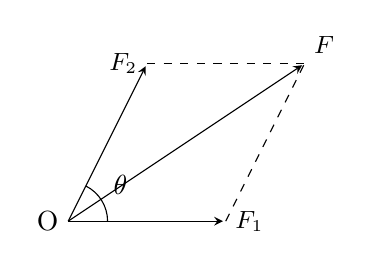
\begin{tikzpicture}
    \draw [->,>=stealth,shorten >=1pt] (0,0)--(2,0) node [anchor=west]{\small $F_1$};
    \draw [->,>=stealth,shorten >=1pt] (0,0)--(1,2) node [anchor=east]{\small $F_2$};
    \draw [dashed] (1,2) --(3,2);
    \draw [dashed] (2,0)--(3,2);
    \draw [->,>=stealth,shorten >=1pt] (0,0)--(3,2) node [anchor=south west]{\small $F$};
    \draw (0,0) node [anchor=east]{O};
    \draw (0.5,0) arc (0:63.43495:0.5);
    \draw (25:0.5) node [anchor=south west]{$\theta$};
  \end{tikzpicture}
  \caption{力的合成}
\end{figure}

由余弦定理容易得到合力与分力的数量关系如下:
\begin{equation}
  F=\sqrt{F_1^2+F_2^2+2F_1F_2\cos\theta}
  \label{eq:cosine law}
\end{equation}

由于夹角范围 $0\leqslant \theta \leqslant \pi$ ,所以$\cos\theta$ 是单调递减的,因此随两个分力的夹角的增大,合力的大小逐渐减小.当$\theta=0$ 时,合力最小,当$\theta=\pi$ 时,合力最大,即
\begin{equation}
  |F_1-F_2|\leqslant F \leqslant F_1+F_2
  \label{eq:resultant force}
\end{equation}

如果知道了两个分力作为矢量的坐标,也可以使用矢量的坐标运算解决.记$F_1=(x_1,y_1)$,$F_2=(x_2,y_2)$,则合力可以表达为
\begin{equation}
  F=\sqrt{(x_1+x_2)^2+(y_1+y_2)^2}
  \label{eq:coordinate force}
\end{equation}
\subsection{余弦定理的证明}
如果同学们是初学者,则按现行的高中数学教材,还没有学到余弦定理,但是此定理无论在数学还是物理上都是十分重要的,所以这里为同学们加以证明.

首先由勾股定理证明一个结论:$\cos^2\theta+\sin^2\theta=1$.如下图
\begin{figure}[H]
  \centering
  \begin{tikzpicture}
    \draw (0,0) node [anchor=east]{A}--(4,0) node [anchor=west]{B}--(4,3) node [anchor=west]{C}--(0,0)--cycle; 
    \draw (0.8,0) arc (0:37:0.8);
    \draw (18.5:0.8) node [anchor=west] {$\theta$};
  \end{tikzpicture}
  \caption{勾股定理}
  \label{fig:gougu law}
\end{figure}

记边长$BC=a$,$AC=b$,$AB=c$,则由勾股定理得
$$a^2+b^2=c^2$$
对上式,左右同时除以$c^2$,得
$$\Big (\cfrac{a}{c} \Big )^2+\Big (\cfrac{b}{c} \Big )^2=1$$
根据三角函数定义$\sin \theta=\frac{a}{c}$ 和 $\cos\theta=\frac{b}{c}$ 上式可以用三角函数表达为
\begin{equation}
\cos^2\theta+\sin^2\theta=1
  \label{eq:gougu}
\end{equation}

如图\ref{fig:cosine law}所示,记边长$BC=a$,$AC=b$,$AB=c$
\begin{figure}[H]
  \centering
  \begin{tikzpicture}
    \draw (0,0) node [anchor=east]{A}--(1.5,0) node [anchor=north]{D}--(3.5,0) node [anchor=west]{B} -- (1.5,2) node [anchor=south] {C} -- (0,0)--cycle; 
    \draw (1.5,0)--(1.5,2);
    \draw (0.3,0) arc (0:53:0.3);
    \draw (15:0.3) node [anchor= south west] {$\theta$};
    \draw (1.75,-0.3) node [anchor=north] {\small 甲};
  \end{tikzpicture}
  \qquad
  \begin{tikzpicture}
    \draw (0,0) node [anchor=east] {D}--(1.5,0) node [anchor=north]{A}--(4,0) node [anchor=west]{B} -- (0,2) node [anchor=south] {C}--(0,0) -- cycle; 
    \draw (0,2)--(1.5,0);
    \draw (1.8,0) arc (0:127:0.3);
    \draw (1.634,0.268) node [anchor=south west] {$\theta$};
    \draw (2,-0.3) node [anchor=north] {\small 乙};
  \end{tikzpicture}
  \caption{余弦定理}
  \label{fig:cosine law}
\end{figure}

在图\ref{fig:cosine law} 甲所示,由三角函数定义易得$CD=b\sin\theta$,$AD=b\cos\theta$,所以$BD=c-b\cos\theta$,由勾股定理得
$$(b\sin\theta)^2+(c-b\cos\theta)^2=a^2$$
将上式展开得
$$b^2(\cos^2\theta+\sin^2\theta)+c^2-2bc\cos\theta=a^2$$
代入\eqref{eq:gougu}式得
$$b^2+c^2-2bc\cos\theta=a^2$$
对于图\ref{fig:cosine law} 乙所示,当$\theta >90^\circ$ 时,定义正弦函数 $\sin\theta=\sin(\pi-\theta)$,余弦函数$\cos\theta=-\cos(\pi -\theta)$.显然式\eqref{eq:gougu} 仍然满足.由三角函数定义可得$AD=b\cos(\pi -\theta)=-b\cos\theta$,$CD=b\sin(\pi-\theta)=b\sin\theta$,由勾股定理得
$$(c-b\cos\theta)^2+(b\sin\theta)^2=a^2$$
经过简单运算同样得
$$b^2+c^2-2bc\cos\theta=a^2$$
上式就是余弦定理.

\eqref{eq:cosine law}式,可以由余弦定理得到,如下
$$F_1^2+F_2^2-2F_1F_2\cos(\pi-\theta)=F^2$$
代入$\cos(\pi-\theta)=-\cos\theta$,同时再开方,移项得
$$F=\sqrt{F_1^2+F_2^2+2F_1F_2\cos\theta}$$


\subsection{正弦定理的证明}

在物体的受力平衡问题中,特别是三力平衡问题中,三个力构成封闭矢量三角形.这类问题的求解和讨论更多的是归结为解三角形,讨论三角形三个边和角的关系.所以正弦定理就相当必要在这里阐述.

\subsubsection{正弦定理}
如图\ref{fig:zhengxian}所示,记三角形的三个角分别为:A,B和C;对应的三条边分别记为:a,b和c.则有关系
\begin{equation}
  \frac{a}{\sin A}=\frac{b}{\sin B}=\frac{c}{\sin C}
  \label{eq:zhengxian}
\end{equation}

\begin{figure}[H]
  \centering
  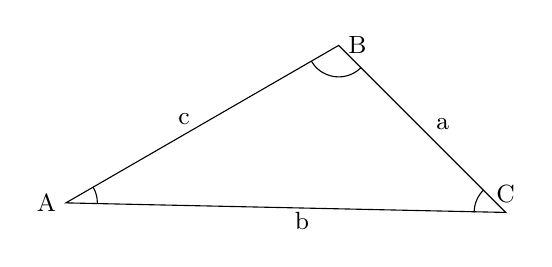
\begin{tikzpicture}
    \draw (0,0) node [anchor=east]{\small A}--++(30:4) node [anchor=west]{\small B}--++(-45:3) node [anchor=south]{\small C}--(0,0)--cycle;
    \draw (30:0.4) arc (30:0:0.4);
    \draw (0,0)++(30:3.6) arc (210:315:0.4);
    \draw (0,0)++(30:4)++(-45:2.6) arc (135:180:0.4);
    \draw (32:2) node [anchor=east]{\small c};
    \draw (30:4)++(-42:1.5) node [anchor=west]{\small a};
    \draw (3,0) node [anchor=north]{\small b};
  \end{tikzpicture}
  \caption{正弦定理}
  \label{fig:zhengxian}
\end{figure}

\subsubsection{正弦定理的证明}

如图\ref{fig:zhengxian1}所示,任何一个三解开必有一个外接圆,由平面几何易知,圆周角是圆心角的一半,在图\ref{fig:zhengxian1}中$OD$垂直于$BC$,由于$OB=OC$所以$OD$又是$\angle BOC$的平分线,则$\angle BOD=A$,由几何关系可得三解形外接圆的半径为

\[
  R=\frac{a}{2\sin A}
\]

同理由其它二个角也可以写出半径
\[
  R=\frac{b}{2\sin B}=\frac{c}{2\sin C}
\]

将三个求半径的式子写到一块,同时乘以$2$化成直径,则得到正弦定理

\[
  2R=\frac{a}{\sin A}=\frac{b}{\sin B}=\frac{c}{\sin C}
\]


\begin{figure}[H]
  \centering
  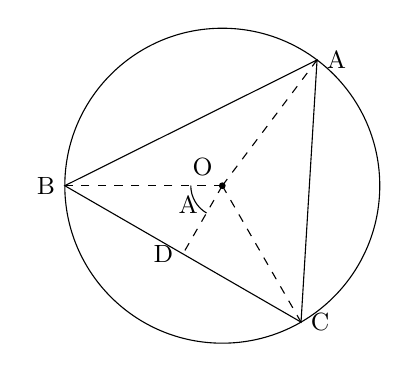
\begin{tikzpicture}
    \draw (0,0) circle [radius=2];
    \draw [dashed] (0,0)--(53:2) node [anchor=west]{\small A};
    \draw [dashed] (0,0)--(-60:2) node [anchor=west]{\small C};
    \draw [dashed] (0,0)--(180:2) node [anchor=east]{\small B};
    \draw (53:2)--(180:2)--(-60:2)--(53:2)--cycle;
    \draw[dashed] (0,0)--(-120:1) node [anchor=east]{\small D};
    \filldraw (0,0) circle [radius=1pt] node [anchor=south east]{\small O};
    \draw (180:0.4) arc (180:240:0.4);
    \draw (210:0.5) node {\small A};
  \end{tikzpicture}
  \caption{正弦定理证明}
  \label{fig:zhengxian1}
\end{figure}
\subsection{注意事项}
力是矢量,遵守平行四边行定则 ,但是在考虑实际问题时并不是所有的情况都可以使用力的合成.能够进行力的合成的情况,只能是所谓的共点力.

共点力:如果几个力共同作用在\CJKunderwave{同一点} 上,或者虽不作用在同一点上,但是它们的\CJKunderwave{作用线}交于一点,这样的一组力叫做共点力.
